\chapter{Annexes}
\label{chap:annexes}

\section{Liste des endpoints REST}
\label{ann:endpoints}

L'API expose environ 85 endpoints répartis sur 17 contrôleurs. Le
tableau~\ref{tab:endpoints} en donne une vue synthétique.

\renewcommand{\arraystretch}{1.2}\footnotesize
\begin{longtable}{L{3.6cm} L{10.4cm}}
\caption{Synthèse des endpoints REST}\label{tab:endpoints}\\
\toprule
\textbf{Ressource} & \textbf{Endpoints} \\
\midrule \endfirsthead
\toprule \textbf{Ressource} & \textbf{Endpoints} \\ \midrule \endhead
\texttt{/api/auth} & POST /register, POST /login, PATCH /users/\{id\}/roles, DELETE /users/\{id\}/roles \\
\texttt{/api/tenants} & GET, GET /\{id\}, POST /register, PUT /\{id\}, DELETE /\{id\} \\
\texttt{/api/users} & GET, GET /\{id\}, GET /email/\{email\} \\
\texttt{/api/actors} & GET, GET /\{id\}, GET /user/\{userId\}, GET /role/\{role\}, POST /user/\{userId\}, DELETE /\{id\} \\
\texttt{/api/businesses} & GET, POST, GET /\{id\}, GET /domain/\{domain\}, GET /search, PUT /\{id\}, DELETE /\{id\} \\
\texttt{/api/business-rules} & GET, GET /\{id\}, GET /business/\{businessId\}, POST /business/\{businessId\}, PUT /\{id\}, DELETE /\{id\} \\
\texttt{/api/service-catalogues} & GET, GET /\{id\}, GET /business/\{businessId\}, GET /available, GET /search, POST /business/\{businessId\}, PUT /\{id\}, DELETE /\{id\} \\
\texttt{/api/service-requests} & GET, GET /\{id\}, GET /consumer/\{id\}, GET /provider/\{id\}, GET /status/\{status\}, POST /consumer/\{id\}/provider/\{id\}/catalogue/\{id\}, PATCH /\{id\}/accept, /start, /fulfill, /cancel, DELETE /\{id\} \\
\texttt{/api/invoices} & GET, GET /\{id\}, GET /status/\{status\}, GET /service-request/\{id\}, POST /service-request/\{id\}, PATCH /\{id\}/pay, /cancel, DELETE /\{id\} \\
\texttt{/.../messages} & GET, POST, GET /unread-count, PATCH /read-all, DELETE /\{messageId\} \\
\texttt{/api/notifications} & GET, GET /unread-count, PATCH /\{id\}/read, PATCH /read-all, DELETE /\{id\} \\
\texttt{/api/portfolios} & GET, GET /\{id\}, GET /actor/\{id\}, POST /actor/\{id\}, PATCH /\{id\}/businesses/\{bid\}, DELETE /\{id\}/businesses/\{bid\}, DELETE /\{id\} \\
\texttt{/api/resources} & GET, GET /\{id\}, GET /business/\{id\}, POST /business/\{id\}, PUT /\{id\}, DELETE /\{id\} \\
\texttt{/api/media} & GET, GET /\{id\}, GET /business/\{id\}, GET /type/\{type\}, POST /business/\{id\}, PUT /\{id\}, DELETE /\{id\} \\
\texttt{/api/currencies} & GET, GET /validate/\{code\} \\
\texttt{/api/analytics} & GET /tenants/\{tenantId\}/kpis \\
\texttt{/api/audit} & GET /service-requests/\{id\}, GET /actors/\{id\}, GET /trace/\{traceId\}, GET /tenants/\{id\} \\
\bottomrule
\end{longtable}

\section{Exemple de log structuré}

\begin{lstlisting}[language=json,caption={Log structuré au format JSON (proposition)},captionpos=b]
{
  "timestamp": "2025-05-04T10:05:23Z",
  "level": "INFO",
  "tenant_id": "550e8400-e29b-41d4-a716-446655440000",
  "trace_id": "7e9a8b7c-6d5e-4f3a-2b1c-9d8e7f6a5b4c",
  "actor_id": "actor_123",
  "service": "BusinessService",
  "operation": "createBusiness",
  "duration_ms": 145,
  "http_status": 201
}
\end{lstlisting}

\section{Capture Swagger UI}
\label{ann:swagger}

\begin{figure}[htbp]
  \centering
  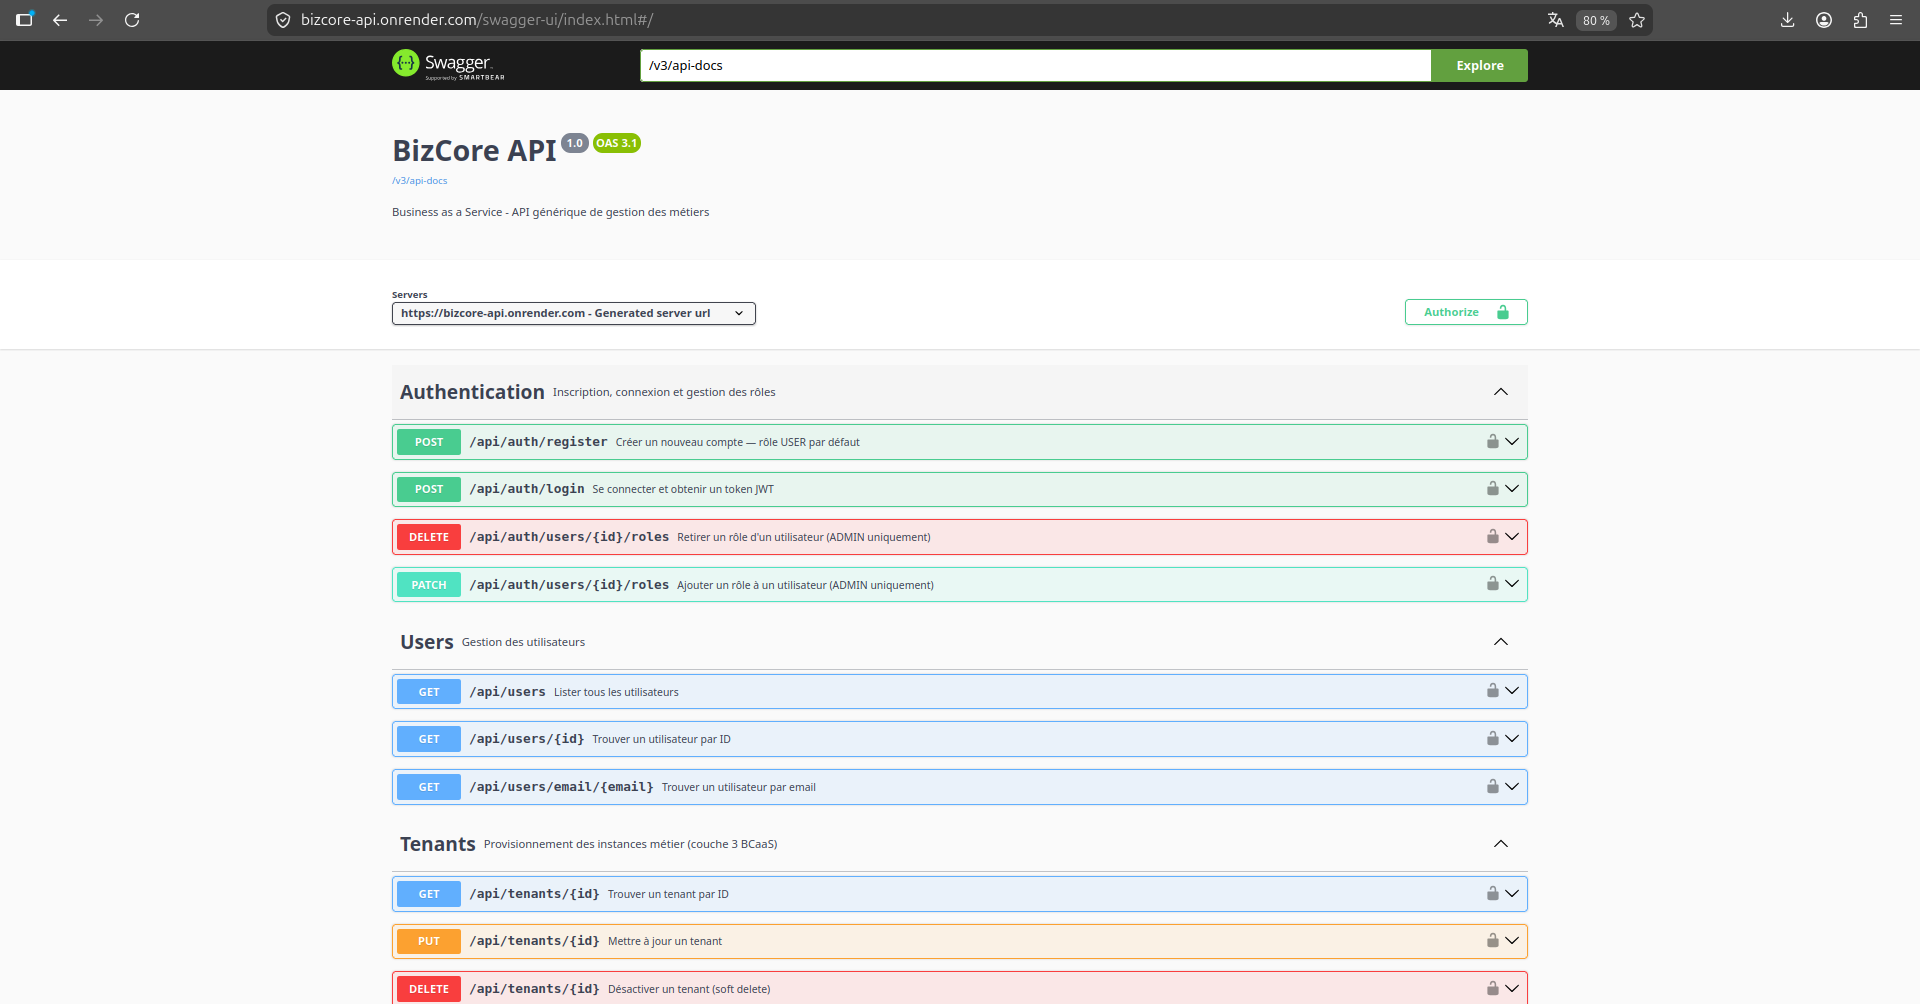
\includegraphics[width=\textwidth]{figures/Screenshots/SWAGGER.png}
  \caption{Documentation interactive Swagger UI}
  \label{fig:swagger}
\end{figure}

\section{Extraits de code significatifs}

\begin{lstlisting}[language=Java,caption={TenantContext (ThreadLocal)},captionpos=b]
public final class TenantContext {
    private static final ThreadLocal<UUID> CURRENT_TENANT = new ThreadLocal<>();
    public static void setTenantId(UUID tenantId) { CURRENT_TENANT.set(tenantId); }
    public static UUID getTenantId() { return CURRENT_TENANT.get(); }
    public static void clear() { CURRENT_TENANT.remove(); }
}
\end{lstlisting}

\begin{lstlisting}[language=Java,caption={Lecture tenant-aware dans un service},captionpos=b]
UUID tenantId = TenantContext.getTenantId();
if (tenantId != null) {
    return serviceRequestRepository.findAllByTenantId(tenantId, pageable);
}
\end{lstlisting}
